\documentclass{article}
\usepackage{amsfonts, amsmath, amssymb, amsthm} % Math notations imported
\usepackage{enumitem}
\usepackage[margin=1in]{geometry}
\usepackage{graphicx}
\graphicspath{{./images}}

\newtheorem{thm}{Theorem}
\newtheorem{prop}[thm]{Proposition}
\newtheorem{cor}[thm]{Corollary}

% title information
\title{Math 154 HW7}
\author{Neo Lee}
\date{05/31/2023}

% main content
\begin{document} 

% placing title information; comment out if using fancyhdr
\maketitle 

\textbf{Problem 1.}
The complement $\overline{G}$ of a graph $G$ is the graph on the same vertex set where $\{u,v\}\in E(\overline{G})$ if and only if $\{u,v\}\not\in E(G)$. 
(In other words, to obtain the complement $\overline{G}$ of $G$, we fill in all the edges missing from $G$ to form a complete graph, then delete the edges originally present in G.)
\begin{enumerate}[label=(\alph*)]
    \item 
    \begin{prop}
        For every graph $G$ on 11 or more vertices, at most one of G and $\overline{G}$ can be planar.
    \end{prop}
    \begin{proof}
        Assume for the sake of contradiction that both $G$ and $\overline{G}$ can be planar.
    
        Let $n$ be the number of vertices in $G$.
        Since $E(G)$ and $E(\overline{G})$ are disjoint, $E(G) \cup E(\overline{G}) = E(K_n)$.
        Assume without loss of generality that $|E(G)| \ge |E(\overline{G})|$.
        Then $|E(G)| \ge \frac{1}{2} |E(K_n)| = \frac{1}{4} n(n-1)$.
        Performing simple algebric operations, we get
        \begin{align*}
            \frac{1}{4} n(n-1) \le |E(G)| & \le 3|V(G)| - 6 \\
            \frac{1}{2} n^2 - \frac{13}{2} n + 12 & \le 0.
        \end{align*}
        The above inequality is false when $n \ge 11$. Hence, contradiction.
    \end{proof}

    \item 
    Give an example of a graph $G$ on 11 or more vertices where both $G$ and $\overline{G}$ are nonplanar.
    \begin{proof}[Solution]
        Let $G$ be a graph with 12 vertices and 33 arbitrary edgees.
    \end{proof}
\end{enumerate}
\bigbreak

\textbf{Problem 2.}
Determine whether the graph G below is planar or not planar. 
If it is planar, prove it by explicitly drawing a planar embedding of $G$. 
If it is not planar, use Kuratowski's Theorem: identify a subgraph that is a subdivision of $K_5$ or $K_{3,3}$, and draw $G$ with that subgraph clearly highlighted.
\begin{proof}[Solution]
    The induced subgraph with vertices of all the boundary vertices (colored in blue, green, red) is a subdivision of $K_{3,3}$.
    Contract the yellow vertices and we will get a $K_{3,3}$ (blue and red are the two partitions). Hence, $G$ is not planar.
    \begin{figure}[h]
        \centering
        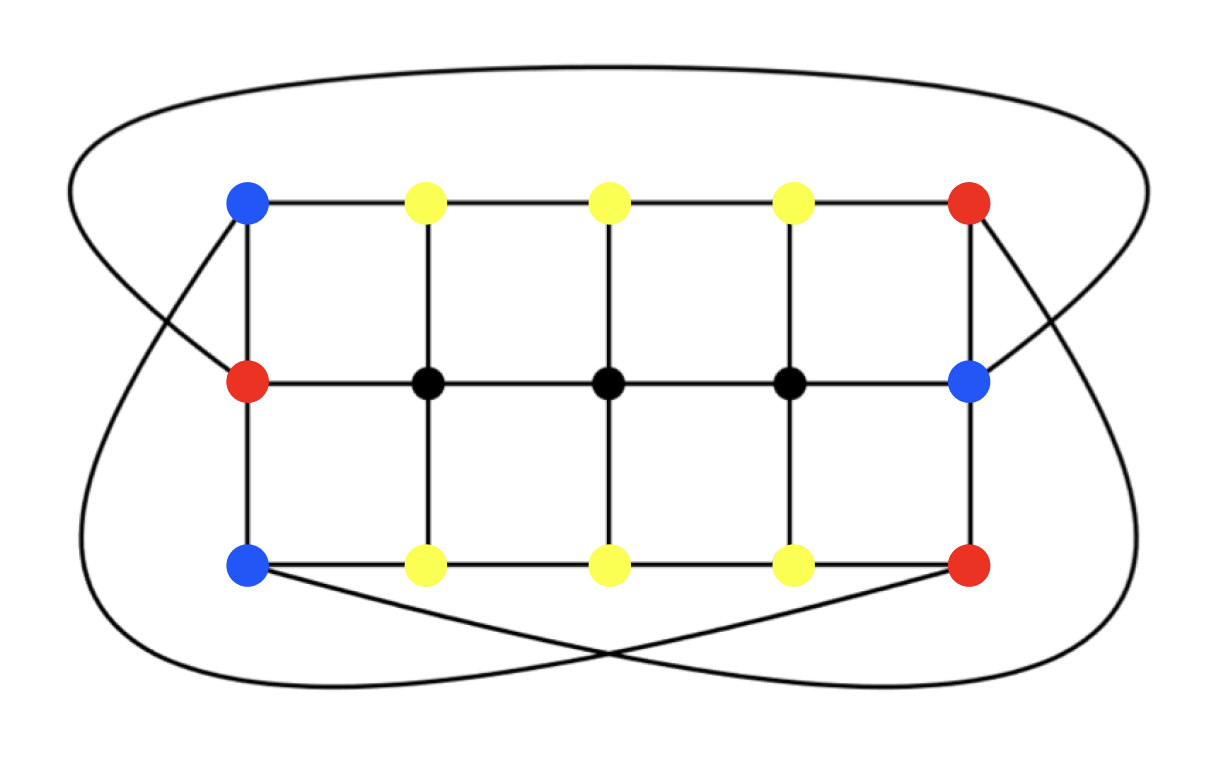
\includegraphics[scale=0.3]{graph.png}
        \caption{Graph $G$}
    \end{figure}
\end{proof}
\bigbreak

\textbf{Problem 3.}
\begin{prop}
    Every triangle-free planar graph is 4-colorable.
\end{prop}
\begin{proof}
    Let $n$ be the number of vertices in the graph. Let an arbitrary triangle-free planar graph $G$,
    \begin{align*}
        & \quad\frac{1}{2}\sum_{v\in V(G)} d(v) = |E(G)| \le \frac{4}{4-2}(n - 2) = 2n - 4 \\ 
        & \Rightarrow \frac{1}{2}\sum_{v\in V(G)} d(v) \le 2n - 4 \\ 
        & \Rightarrow \sum_{v\in V(G)}d(v) \le 4n-8 \\ 
        & \Rightarrow \frac{\sum_{v\in V(G)}d(v)}{n} \le 4-\frac{8}{n} \\ 
        & \Rightarrow \emph{average degree} < 4 \\ 
        & \Rightarrow \exists w \in V(G), d(w) \le 3.
    \end{align*}

    Since every subgraph of $G$ is also triangle-free planar, every subgraph of $G$ has a vertex of degree at most 3.
    Hence, $G$ is 4-degenerate and thus 4-colorable.
\end{proof}
\end{document}